
\scsection{Введение в Технологию OSTIS}
\label{intro_ostis}

\begin{SCn}

\scnsectionheader{\currentname}

\scnstartsubstruct

\scnheader{Технология OSTIS}
\scnidtf{OSTIS}
\scnidtf{\uline{Открытая технология} проектирования \uline{совместимых} интеллектуальных систем}
\filemodetrue
\scnrelfromvector{предпосылки создания}{решение любой актуальной сложной (комплексной) задачи (понимание изображений, понимание текстов и речи, управление предприятиями и т.д.) требует комбинации в рамках системы различных \uline{видов знаний} (не только фактов, но и логических утверждений, ситуаций, событий, алгоритмов, т.д.) и различных \uline{моделей решения задач} (нейросетевых, логических, статистических моделей, классических алгоритмов и т.д.). При этом заранее нельзя сказать, какой именно набор понадобится для решения конкретной задачи.;
в настоящее время существуют системы, которые частично решают задачу интеграции различных моделей, однако такие системы делаются \uline{монолитными} и проектируются под \uline{конкретную задачу}. Разработка таких систем стоит огромных ресурсов, при этом развивать такие системы для решения других задач практически не представляется возможным, приходится делать все заново.}
\filemodefalse
\scnaddlevel{1}
\scnnote{В контексте \textit{Технологии OSTIS} мы считаем, что \uline{интеллектуальной} является не та система, которая может решить конкретную задачу (даже интеллектуальную), а та система, которая может легко \uline{обучаться} решению новых задач без существенных затрат.}
\scnaddlevel{-1}
\filemodetrue
\scnrelfromvector{принципы, лежащие в основе}{В основе \textit{Технологии OSTIS} лежит универсальный способ представления информации, названный \textit{SС-кодом}. В основу \textit{SC-кода} положены основные формализмы дискретной математики (теория множеств и теория графов), что обеспечивает как универсальность и унифицированность представления (можно представить любую информацию одинаковым образом), так и удобство обработки и восприятия человеком.;
Базовый \textit{Алфавит SC-кода} состоит всего из 5 элементов, на основе которых строятся все более сложные конструкции. При этом с помощью \textit{SC-кода} описываются не только знания системы, но и модели решения задач и даже интерфейс системы. Можно провести аналогию с тем, как из базового ограниченного набора элементарных частиц строятся различные вещества и далее различные объекты любой сложности.; 
Системы, построенные на основе \textit{Технологии OSTIS} (ostis-системы) состоят из \textit{базы знаний}, \textit{решателя задач} и \textit{интерфейса} взаимодействия с внешним миром (не обязательно пользовательского).;
\textit{База знаний ostis-системы} может описывать любые виды знаний, при этом легко дополняться новыми знаниями и новыми видами знаний.;
\textit{Решатель задач ostis-системы} основан на многоагентном подходе и позволяет легко интегрировать и комбинировать любые модели решения задач.;
\textit{Интерфейс ostis-системы} представляет собой совокупность специального вида \textit{базы знаний} и \textit{решателя задач}, т.е. также описывается средствами SC-кода.
}
\scnrelfromvector{преимущества}{В \uline{любую} ostis-систему без каких-либо \uline{накладных расходов} можно бесшовно \uline{интегрировать} любые \uline{знания} и \uline{модели решения задач} (по принципу plug\&play). Таким образом, не важно, что система умеет в данный момент, ее всегда можно переобучить на решение другой задачи.;
Разрабатываемые \uline{компоненты} ostis-систем \uline{универсальны} (могут использоваться в совершенно разных системах) и \uline{совместимы} между собой. Это означает, что можно накапливать \uline{библиотеку компонентов} и \uline{использовать компоненты повторно}, таким образом, сильно \uline{сокращается время разработки} каждой следующей системы. Например, в настоящее время универсальная часть (ядро) баз знаний позволяет сократить сроки разработки базы знаний новых систем на 40-60\%.;
За счет того, что вся система описывается средствами SC-кода, она может анализировать сама себя, искать в себе ошибки, оптимизировать собственную работу (обладает рефлексивностью). Рефлексивность считается одним из ключевых признаков интеллекта, даже люди далеко не всегда обладают рефлексивностью.;
За счет наличия базового \textit{Алфавита SC-кода} и возможности полного описания \textit{компьютерной системы} средствами \textit{SC-кода} возникает возможность сделать \textit{ostis-системы} полностью платформенно-независимыми (разделить модель системы и платформу интерпретации таких моделей). То есть разработка ostis-системы сводится к разработке ее модели и выполняется независимо не только от операционной системы, но и в принципе от архитектуры компьютера, на котором система работает. Платформа в свою очередь может быть реализована как \uline{программно} (наподобие виртуальной машины), так и \uline{аппаратно}.;
Как следует из предыдущего пункта, \textit{Технология OSTIS} является основной для нового типа компьютеров -- \uline{\textit{семантических компьютеров}}. В отличие от других компьютеров с нетрадиционной архитектурой (в том числе суперкомпьютеров), для которых не всегда понятно, как именно их использовать, для семантических компьютеров уже готова технология и конкретные системы, которые будут на них работать.;
За счет используемого в \textit{Технологии OSTIS} подхода к обработке информации (особого рода многоагентного подхода) ostis-системы оказываются изначально ориентированы на \uline{параллельную обработку информации}, в том числе, поддержку ее на аппаратном уровне (в рамках семантического компьютера).}
\filemodefalse
\scnaddlevel{1}
    \scntext{вывод}{Таким образом, по сравнению с традиционными технологиями, \textit{Технология OSTIS} позволяет при той же скорости обучения разработчиков и трудоемкости разработки новых компонентов значительно снизить сроки разработки систем за счет повторного использования компонентов и легкости их интеграции. При этом производительность \textit{ostis-системы} по сравнению с аналогичной традиционной системой в общем случае может оказаться ниже, но данная проблема будет решена при переходе на семантические компьютеры.

    При необходимости, \textit{ostis-система} может включать не только компоненты, разработанные на основе \textit{Технологии OSTIS}, но и легко интегрироваться с любыми другими системами и интегрировать другие компоненты посредством специального протокола обмена информацией и/или программного интерфейса (API). Такие компоненты не будут в полной мере обладать некоторыми важными свойствами ostis-систем (например, рефлексивностью) но это позволит заимствовать современные разработки и решить проблему производительности при решении наиболее ресурсоемких задач (например, при обучении нейросетей).
    }
\scnaddlevel{-1}
\scnnote{Важно отметить, что \uline{\textit{OSTIS} -- не конкретная интеллектуальная система} или способ решения задач какого-либо класса, это \uline{технология разработки интеллектуальных систем}, каждая из которых в свою очередь в каждый конкретный момент будет решать задачи определенного класса. При этом ключевые преимущества \textit{OSTIS} заключаются не в принципиально новых функциональных возможностях разрабатываемых систем (большинство \textit{ostis-систем} могут быть реализованы современными традиционными средствами), а в том, насколько легко можно \uline{модифицировать и развивать} разрабатываемые системы, адаптировать их под новые задачи, а также в том, насколько эффективно можно \uline{накапливать и использовать полученные компоненты} при разработке новых систем, снижая при этом сроки и трудоемкость их разработки.
}
\filemodetrue
\scnrelfromvector{текущий состав}{программная реализация платформы (модели семантического компьютера), которая лежит в основе каждой ostis-системы. Может использоваться как при разработке web-приложений, так и настольных и мобильных приложений.;
постоянно пополняемая \textit{Библиотека компонентов баз знаний ostis-систем}, включая универсальное \textit{Ядро баз знаний ostis-систем}. В текущий момент наличие данной библиотеки позволяет сократить сроки разработки баз знаний на 40-60\%.;
постоянно пополняемая \textit{Библиотека компонентов решателей задач ostis-систем}, включая механизмы поиска информации и некоторые модели решения задач, среди которых выделяется соответствующее \textit{Ядро решателей задач ostis-систем}. В настоящее время на первых этапах разработки системы оказывается достаточным использовать только \textit{Ядро решателей задач ostis-систем} и не разрабатывать дополнительно никаких компонентов.;
комплекс \textit{Средств информационной поддержки разработчиков ostis-систем} (включая описание самих моделей, а также методики и руководства), оформленных в виде интеллектуальной \textit{Метасистемы IMS.ostis} (IMS) и доступный онлайн \url{https://ims.ostis.net.}}

\scnrelfromvector{текущее применение}{на основе \textit{Технологии OSTIS} силами студентов и аспирантов активно развивается большое число открытых прототипов обучающих и справочных систем, которые можно найти на \url{https://github.com/ostis-apps};
разработки на основе \textit{Технологии OSTIS} успешно внедрены на ОАО ``Савушкин продукт''  при разработке системы информационного обслуживания сотрудников и при разработке компонентов систем контроля качества продукции;
\textit{Технология OSTIS} позволит значительно более эффективно реализовать анализ естественного языка (включая речь), в том числе для чат-ботов, синхронного перевода и речевых ассистентов. В настоящее время выполняется ряд проектов по данной тематике.}
\filemodefalse
\scntext{планы развития}{Предполагается, что в ближайшем будущем \textit{Метасистема IMS.ostis} и другие \textit{ostis-системы} будут объединены в распределенную облачную \textit{ostis-систему}, названную \textit{Экосистемой OSTIS}. Общая архитектура экосистемы показана на рисунке \textit{Архитектура Экосистемы OSTIS}. При этом все \textit{ostis-системы} в составе \textit{Экосистемы OSTIS} будут в каждый момент времени совместимы между собой, при этом совместимость будет контролироваться автоматически. Любой желающий сможет внести свой вклад в развитие любой из ostis-систем в составе \textit{Экосистемы OSTIS}, в первую очередь -- \textit{Метасистемы IMS.ostis}, при этом вклад будет автоматически верифицироваться и оцениваться. В то же время, как видно из представленной архитектуры, владельцы \textit{ostis-систем} смогут самостоятельно выбирать, какой частью своей информации они готовы поделиться с другими пользователями \textit{Экосистемы OSTIS}, персональная же часть информации будет гарантированно защищена.}

\scnheader{Архитектура Экосистемы OSTIS}
\scneqimage{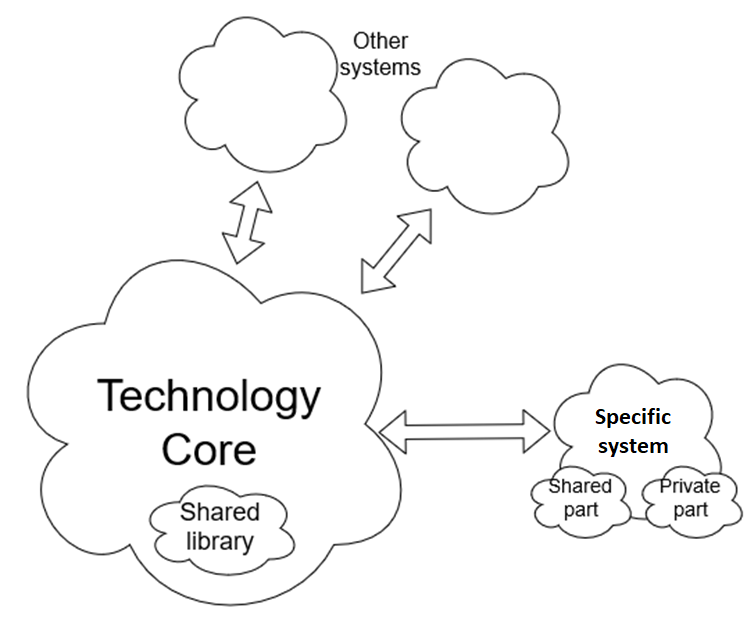
\includegraphics[width=0.6\textwidth]{figures/chapter0/ecosystem.png}}

\scnheader{Технология OSTIS}
\scnrelfromvector{текущие проекты}{Проект Экосистема OSTIS;Проект Метасистема IMS.ostis;Проект Семейство различных вариантов реализации универсального интерпретатора семантических моделей интеллектуальных систем\\
\scnaddlevel{1}
    \scnrelfromlist{подпроект}{Проект Программно реализованный на современных компьютерах универсальный интерпретатор семантических моделей интеллектуальных систем;Проект Семантический ассоциативный компьютер}
\scnaddlevel{-1}
;Проект Комплекс совместимых средств проектирования интеллектуальных систем\\
\scnaddlevel{1}
    \scnrelfromlist{подпроект}{Проект Встраиваемая типовая интеллектуальная система комплексной поддержки проектирования баз знаний;Проект Интеллектуальная система комплексной поддержки проектирования решателей задач интеллектуальных систем;Проект Интеллектуальная система комплексной поддержки проектирования вербальных интерфейсов интеллектуальных систем;Проект Интеллектуальная система комплексной поддержки проектирования невербальных интерфейсов}
\scnaddlevel{-1}
;Проект Семейство совместимых интеллектуальных справочных, обучающих и help-систем\\
\scnaddlevel{1}
    \scnrelfromlist{подпроект}{Проект Специализированные средства разработки совместимых интеллектуальных справочных, обучающих и help-систем различного назначения;Проект Комплекс семантически совместимых интеллектуальных справочных и обучающих систем по всем дисциплинам среднего образования;Проект Комплекс семантически совместимых интеллектуальных справочных и обучающих систем по всем дисциплинам, являющихся базовыми при подготовке инженеров по информационным специальностям;Проект Комплекс семантически совместимых интеллектуальных справочных и обучающих систем по всем специальным дисциплинам специальности ''Искусственный интеллект''{};Проект Семейство совместимых интеллектуальных справочных и обучающих систем по стандартам различного вида}
\scnaddlevel{-1}
;Проект Семейство совместимых интеллектуальных корпоративных систем ситуационного управления\\
\scnaddlevel{1}
    \scnrelfromlist{подпроект}{Проект Интеллектуальная корпоративная система ситуационного управления предприятием рецептурного производства;Проект Интеллектуальная корпоративная система ситуационного управления деятельностью выпускающей кафедры технического вуза}
\scnaddlevel{-1}
}
\scnrelfromvector{будущие проекты}{
Проект Семейство совместимых интеллектуальных систем автоматизации проектирования в различных областях;Проект Семейство совместимых порталов знаний\\
\scnaddlevel{1}
    \scnrelfrom{подпроект}{Проект Портал научных знаний по искусственному интеллекту}
\scnaddlevel{-1}
;Проект Семейство совместимых интеллектуальных систем экскурсионного обслуживания;Проект Семейство совместимых интеллектуальных геоинформационных систем;Проект Семейство совместимых интеллектуальных робототехнических систем и специализированных средств их разработки;Проект Семейство совместимых интеллектуальных систем персонального обслуживания и мониторинга\\
\scnaddlevel{1}
    \scnrelfromlist{подпроект}{Проект Интеллектуальная система персонального обслуживания и мониторинга пользователей и разработчиков компьютерных систем, входящих в Экосистему OSTIS;Проект Интеллектуальный персональный ассистент по взаимодействию с традиционными internet-системами и их пользователями;Проект Интеллектуальная система персонального комплексного медицинского мониторинга и контроля}
\scnaddlevel{-1}
}

\scnheader{смысловое представление информации}
\scnrelfromset{принципы, лежащие в основе}{
\scnfileitem{Каждый синтаксически элементарный (атомарный) фрагмент представленной информации является обозначением некоторой сущности, которая может быть реальной или абстрактной, конкретной (фиксированной, константной) или произвольной (переменной), постоянной или временной, четкой (достоверной) или нечеткой (недостоверной с возможным дополнительным уточнением степени правдоподобности).}
	\scnaddlevel{1}
\scntext{следовательно}{В состав смыслового представления информации не могут входить буквы, слова, словосочетания, разделители, ограничители}
	\scnaddlevel{-1}
;\scnfileitem{В рамках смыслового представления информации отсутствует синонимия (пары синонимичных знаков), омонимия  (омонимичные знаки), семантическая эквивалентность (пары семантически эквивалентных информационных конструкций), т.е. отсутствует любая форма дублирования информации, а также отсутствует неоднозначность соотношения между знаками и их денотатами.}}
	\scnaddlevel{1}
\scntext{следовательно}{Смысловое представление информации не может выглядеть как цепочка (строка, последовательность) синтаксически элементарных фрагментов, поскольку каждая описываемая сущность и взаимно однозначно соответствующий ей ее знак может быть связана не с двумя, а с любым количеством описываемых сущностей. Другими словами, смысловое представление информации является нелинейной (графовой) информационной конструкцией.}
		\scnaddlevel{1}
\scntext{следовательно}{Если внутреннее представление информации в памяти компьютерной системы является смысловым представлением, то обработка информации в такой памяти носит графодинамический характер и сводится не к изменению состояния элементов памяти, а к изменению конфигурации связей между ними.}
	\scnaddlevel{-2}
\scnnote{Ключевая проблема современного этапа развития общей теории интеллектуальных компьютерных систем и технологии их разработки – это проблема обеспечения \textbf{\textit{семантической совместимости}} 
\begin{enumerate}
	\item различных видов знаний, входящих в состав баз знаний интеллектуальных компьютерных систем;
	\item различных видов моделей решателей задач;
	\item различных интеллектуальных компьютерных систем в целом;
\end{enumerate}
Для решения этой проблемы очевидно необходима унификация (стандартизация) формы представления знаний в памяти интеллектуальных компьютерных систем. Предлагаемым нами подходом для такой унификации и является ориентация на \textbf{смысловое представление информации (знаний)} в памяти интеллектуальных компьютерных систем. Основой предполагаемого нами подхода к обеспечению высокого уровня обучаемости т семантической совместимости интеллектуальных компьютерных систем, а также к разработке стандарта интеллектуальных компьютерных систем является унификация \textbf{смыслового представления информации (знаний)} в памяти интеллектуальных компьютерных систем и построение глобального \textbf{смыслового пространства} знаний.}
\scnaddlevel{1}
\scnnote{Информация в знаковой конструкции в основном содержится не в самих знаках (в их структуре), а в связях между знаками. При этом существенно, чтобы эти связи (синтаксические связи) имели четкую смысловую (семантическую) интерпретацию. 
Если структура знаков содержит информацию об обозначаемой сущности всегда можно заменить на «бесструктурные» знаки, которые имеют семантическую окружность} 

\scnheader{семантическая сеть}
\scnsubset{смысловое представление информации}
\scnexplanation{Семантическая сеть нами рассматривается не как красивая метафора сложноструктурированных знаковых конструкций, а как формальное уточнение понятия смыслового представления информации, как принцип представления информации, лежащей в основе нового поколения компьютерных языков и самих компьютерных систем – графовых языков и графовых компьютеров.}

\scnheader{семантическая сеть}
\scnsubset{знаковая конструкция}
\scnexplanation{Семантическая сеть – это знаковая конструкция, обладающая следующими свойствами:
	\begin{scnitemize}
		\item «внутренняя» структура (строение) знаков, входящих в семантическую сеть; не требуется учитывать при ее семантическом анализе (понимании)
		\item Смысл семантической сети определяется денотационной семантикой всех входящих в нее знаков и конфигурацией связей инцидентности этих знаков
		\item Из двух инцидентных знаков, входящих в семантическую сеть, один является знаком связи
		\item Синонимия, омонимия
	\end{scnitemize}
}

\scnheader{семантическая сеть}
\scnrelfrom{предлагаемый подход}{\textbf{SC-код}}
	\scnaddlevel{1}
	\scnidtf{Предлагаемое в рамках \textit{Технологии OSTIS} уточнение понятия \textit{семантической сети}}
	\scnaddlevel{-1}
\scnsuperset{SC-код}
	\scnaddlevel{1}
	\scnidtf{Semantic Computer Code}
	 \scnrelfromlist{смотрите}{Раздел 0.3.2; Раздел 2.1.1.1}
	 
\scnheader{многоагентная система}
\scnsubset{кибернетическая система}
\scnexplanation{Кибернетическая система, представляющая собой множество кибернетических систем, способных коммуницировать, т.е. обмениваться информацией друг с другом (причем не обязательно каждый с каждым)}

\scnheader{агент*}
\scnidtf{агент многоагентной системы*}

\scnheader{внешняя среда*}
\scnidtf{внешняя среда кибернетической системы}

\scnheader{память*}
\scnidtf{внутренняя (информационная) среда кибернетической системы}
\scnnote{Не каждая кибернетическая система (в том числе многоагентная система) имеет явно выделенную память, являющуюся хранилищем накапливаемой информации, накапливаемого опыта.}

\scnheader{многоагентная система}
\scnsubdividing{многоагентная система без общей памяти;многоагентная система с общей памятью}
\scnsubdividing{многоагентная система, в которой управление агентами осуществляется только путем обмена сообщениями между ними;многоагентная система, в которой управление агентами осуществляется через общую для них память}
\scnsubdividing{многоагентная система с централизованным управлением агентами;многоагентная система с децентрализованным управлением агентами}
\scnsubdividing{многоагентная система, в которой областью деятельности всех ее агентов является только внешняя среда этой системы;многоагентная система, в которой областью деятельности ее агентов является как внешняя среда, так и память этой системы\\
	\scnaddlevel{1}	
\scnnote{некоторые агенты такой системы могут работать только в памяти}}
	\scnaddlevel{-1}
	
\scnheader{агентно-ориентированная модель обработки информации в памяти}
\scnidtf{агентно-ориентированная модель решения задач}	
\scnidtf{агентно-ориентированная архитектура решателя задач, представляющая собой многоагентную систему, в которой управление ее агентами и областью деятельности агентов является общая для них память}
	\scnaddlevel{1}
	\scntext{следовательно}{условиями инициирования каждого указанного агента является возникновение в указанной памяти соответствующего вида ситуации или события}
	\scnaddlevel{-1}
\scnreltoset{пересечение}{многоагентная система, в которой управление агентами осуществляется через общую для них память;
многоагентная система с децентрализованным управлением агентами;
многоагентная система, в которой областью деятельности ее агентов является как внешняя среда, так и память этой системы}

\scnheader{агентно-ориентированная модель обработки информации в памяти}
\scnrelfromset{принципы, лежащие в основе}{
\scnfileitem{Распределение целенаправленной деятельности между агентами, выполняющими различные действия в памяти, осуществляется на основе генерируемой в базе знаний иерархической системы, описывающей связь (сведение) инициированных целей (задач) с подцелями (подзадачами).}
;\scnfileitem{Условием инициирования агента является появление в базе знаний формулировки той цели (задачи), которая, во-первых, инициирована, а, во-вторых, либо может быть полностью достигнута (решена) этим агентом, либо может быть этим агентом достигнута (решена) частично.}
;\scnfileitem{В результате частичного достижения (решения) некоторой цели (задачи) агент может сгенерировать новые подцели (подзадачи).}
;\scnfileitem{Таким образом, условием инициирования агента обработки информации (базы знаний) является появление соответствующей этому агенту ситуации или соответствия.}}
\scnrelfrom{предлагаемый подход}{\textbf{абстрактная sc-машина}}
	\scnaddlevel{1}
	\scnidtf{Предлагаемое в рамках технологии OSTIS уточнение понятия агентно-ориентированной модели обработки информации в памяти}
	\scnaddlevel{-1}
\scnsuperset{абстрактная sc-машина}

\scnheader{агентно-ориентированная модель обработки информации в памяти}
\scnidtf{многоагентная система}
\scnidtf{многоагентная кибернетическая система}
\scnauthorcomment{Оформление 150 страницы пересмотреть}
\scnnote{Децентрализованное (агентно-ориентированное) управление процессом решения задач в ostis-системах реализуется как на внутреннем уровне (на уровне решателя задач ostis-системы), так и на внешнем уровне (на уровне взаимодействия между ostis-системами)}

\scnheader{стандартизация ostis-систем}
\scnidtf{унификация ostis-систем}
\scnexplanation{Стандартизация ostis-систем включает в себя:
	\begin{scnitemize}
		\item cтандартизацию языка внутреннего представления информации в памяти ostis-систем;
		\item cтандартизация принципов децентрализованного управления обработкой информации в памяти ostis-систем;
		\item cтандартизация языка описания ситуаций и событий (в памяти ostis-систем), которые являются условиями инициирования различных информационных процессов в памяти ostis-систем;
		\item стандартизация базового языка спецификации (описания), программирования агентов, выполняющих соответствующие информационные процессы в памяти ostis-систем;
		\item стандартизация базовых языков ввода/вывода информации в/из памяти ostis-систем.
	\end{scnitemize}}

\scnheader{SC-код}
\scnidtf{Стандарт \textit{смыслового представления} информации в памяти \textit{ostis-системы}, а, точнее, \textit{стандарт семантических сетей}}

\scnheader{абстрактная sc-машина}
\scnidtf{Стандарт \textit{агентно-ориентированной модели обработки информации в памяти ostis-системы}}

\scnheader{стандартизация}
\scnidtf{унификация}
\scnrelfromset{проблемы текущего состояния}{
\scnfileitem{Разработка и совершенствование стандартов происходит очень медленно}
;\scnfileitem{В разработке и совершенствовании стандартов принимает участие явно недостаточное число профессионалов – не учитываются все мнения}
;\scnfileitem{В разработке и совершенствовании стандарта отсутствует четкая методика формирования консенсуса}
;\scnfileitem{При введении новой версии стандарта отсутствует четкая методика перевода на новую версию стандарта всех систем, разработанных по предыдущей версии}}
\scnaauthorcomment{Нужна ли эта запись?}

\scntext{наш подход}{Стандарт – это перманентно совершенствуемая база знаний, поддержку эволюции которой осуществляет соответствующий портал}

\scnheader{конвергенция знаний в памяти ostis-системы}
\scnrelfromset{принципы, лежащие в основе}{
\scnfileitem{Вводится \uline{универсальный}  базовый язык внутреннего \uline{смыслового} представления знаний в памяти ostis-систем (\textit{SC-код}), по строению к которому все внутренние языки, ориентированные на представление знаний различного вида (логические языки, языки представления методов решения задач (в частности, программ), язык формулировки задач, онтологические языки и многие другие) являются подъязыками \textit{SC-кода}, синтаксис которых полностью совпадает с синтаксисом \textit{SC-кода}.}
;\scnfileitem{Конвергенция различных знаний сводится к согласованию систем понятий, используемых для представления знаний различного вида. Такое согласование направлено на увеличение числа общих понятий, используемых при представлении различных знаний.}}

\scnheader{конвергенция моделей решения задач в ostis-системе}
\scnrelfromset{принципы, лежащие в основе}{
\scnfileitem{Синтаксис языка представления соответствующего класса методов решения задач в памяти – синтаксис sc-кода}
;\scnfileitem{Денотационная семантика описывается в виде соответствующей онтологии и представляется в виде текста sc-кода}
;\scnfileitem{Операционная семантика каждой модели решения задач – коллектив \uline{агентов}. Он может быть иерархическим на основе различных моделей решателей, но есть базовая модель интерпретации \uline{любых} методов – 
	\begin{scnitemize}
	\item Язык SCP
		\begin{scnitemize}
		\item cинтаксис = синтаксис SC-кода
		\item денотационная семантика – процедурный язык программирования в графодинамической памяти
		\item операционная семантика реализуется на уровне прозрачной или \scnauthorcomment{какое слово?} платформе
		\end{scnitemize}
	\item sc-агенты работают в общей среде – (sc-памяти) параллельно, асинхронно на основе ряда правил, позволяющих им не «мешать» друг другу
	\end{scnitemize}}}
	
\scnheader{интеграция знаний в памяти ostis-системы*}
\scnexplanation{Интеграция знаний в памяти ostis-систем сводится к склеиванию (отождествлению) синонимичных знаков}

\scnheader{интеграция моделей решения задач в ostis-системе*}
\scnexplanation{Поскольку модель решения задач, используемая ostis-системой, представлена в памяти ostis-системы как соответствующий вид знаний, интеграция различных моделей решения задач может происходить в ostis-системе точно так же, как и интеграция любых других видов знаний. Кроме того, когда речь идет об интеграции различных моделей решения задач имеется в виду возможность одновременного использования различных моделей решения задач при обработке одни и тех же знаний и, в частности, при решении одной и той же задачи. Такая возможность в ostis-системе обеспечивается \textit{агентно-ориентированной моделью обработки информации} в памяти ostis-системы. Таким образом, такого рода интеграция различных моделей решения задач для ostis-систем является тривиальной.}

\scnheader{ostis-система}
\scnrelfromset{достоинства}{
\scnfileitem{Высокий уровень способности \textit{ostis-системы} осуществлять семантическую интеграцию знаний в своей памяти (в частности, при погружении новых знаний в текущее состояние базы знаний) \uline{обеспечивается} смысловым характером внутреннего кодирования информации,  хранимой в памяти ostis-системы и, в частности, тем, что во внутреннем коде базы знаний \textit{ostis-системы} запущены омонимичные знаки и пары синонимичных знаков.}
;\scnfileitem{Высокий уровень способности интегрировать различные виды знаний в \textit{ostis-системах} \uline{обеспечивается} тем, что каждый язык, ориентированный на представление знаний соответствующего вида является \uline{подъязыком} одного и того же базового языка \textit{SC-кода}.\\
\scnnote{Кроме того можно говорить об иерархии sc-языков}}
;\scnfileitem{Высокий уровень способности интегрировать различные модели решения задач в \textit{ostis-системах} \uline{обеспечивается}:
	\begin{scnitemize}
	\item тем, что все эти модели ориентированы на обработку информации, представленной в \textit{SC-коде}
	\item один и тот же фрагмент базы знаний ostis-системы (т.е. одна и та же конструкция sc-кода) может одновременно обрабатываться несколькими \uline{разными} моделями решения задач
	\item все модели решения задач в ostis-системах интегрируются с помощью одной и той же базовой модели решения задач – \textit{scp-модели решения задач} \scnauthorcomment{(пояснить)}
	\end{scnitemize}}
;\scnfileitem{Высокий уровень обучаемости \textit{ostis-систем} \uline{обеспечивается}:
	\begin{scnitemize}
	\item высоким уровнем семантической гибкости информации, хранимой в памяти ostis-системы, поскольку каждое удаление или добавление синтаксически элементарного фрагмента хранимой информации, а также удаление или добавление каждой связи инцидентности между такими элементами имеет четкую семантическую интерпретацию;
	\item высоким уровнем стратифицированности хранимой информации, что обеспечивается онтологически ориентированной структуризацией базы знаний ostis-системы; 
	\item высоким уровнем рефлексии ostis-системы, что обеспечивается мощными метаязыковыми возможностями языка внутреннего представления информации (знаний) в памяти \textit{ostis-систем}.
	\end{scnitemize}}
;\scnfileitem{Каждая \textit{ostis-система} имеет высокий \textit{уровень обучаемости} (способности к быстрому расширению своих \textit{знаний} и \textit{навыков}) и высокий \textit{уровень социализации} (способности к эффективному участию в деятельности различных коллективов – коллективов, состоящих из \textit{ostis-систем}, и сообществ, состоящих из \textit{ostis-систем} и людей}
	\scnaddlevel{1}
\scnrelfromset{детализация достоинства}{
\scnfileitem{Существуют четкие формальные критерии, определяющие \textit{уровень семантической совместимости} (уровень семантической конвергенции) различных знаний, навыков, целых \textit{ostis-систем} (точнее, баз знаний этих систем). Очевидно, что \textit{уровень семантической совместимости} прежде всего определяется количеством «точек соприкосновения» в сравниваемых \textit{знаниях}, \textit{навыках} и \textit{базах знаний} – это \textit{знаки}, присутствующие \uline{в разных} сравниваемых объектах, но имеющие одинаковые денотаты (т.е. обозначающие одинаковые сущности). При этом среди таких знаков, обозначающих одинаковые сущности и присутствующих в разных сравниваемых объектах особенно важны знаки, обозначающие \textit{понятия}.
Количество таких общих понятий в сравниваемых знаниях, навыках, базах знаний определяет уровень семантической совместимости (уровень согласованности) систем используемых понятий в сравниваемых указанных объектах. Увеличение количества знаков, обозначающих одинаковые сущности и присутствующих в разных сравниваемых объектах, может привести к тому, что в разных указанных сравниваемых объектах будут присутствовать не только семантически эквивалентные знаки, но и семантически эквивалентные целые фрагменты (целые информационные конструкции).
Существенно при этом подчеркнуть, что семантически эквивалентные знаковые конструкции, представленные на внутреннем языке ostis-систем (в SC-коде), в памяти разных ostis-систем всегда являются синтаксически изоморфными графовыми конструкциями, в которых соответствие изоморфизма связывает знаки, хранимые в памяти разных ostis-систем, но обозначающие одинаковые сущности (точнее, одну и ту же сущность). Заметим также, что в рамках памяти каждой индивидуальной \textit{ostis-системы} синонимия знаков и, соответственно, семантическая эквивалентность знаковых конструкций запрещены.}
;\scnfileitem{Благодаря постоянно развиваемым семантическим стандартам \textit{Технологии OSTIS} , которые представлены системой формальных онтологий для самых различных предметных областей, разрабатываемые \textit{ostis-системы} \uline{изначально} имеют достаточно высокий \textit{уровень семантической совместимости} со всеми остальными \textit{ostis-системами}. Более того, в \textit{Технологии OSTIS} выделяется целое ядро всех ostis-систем, содержащее фундаментальные базовые знания и базовые навыки, одинаковые для всех ostis-систем и позволяющее каждой копии этого ядра развиваться (общаться, специализироваться) в любом направлении.}
;\scnfileitem{Каждая ostis-система, взаимодействуя с людьми (пользователями) или с другими ostis-системами, обладает способностью повышать уровень семантической совместимости (взаимопонимания) с ними, а также поддерживать (сохранять) высокий уровень такой совместимости в условиях (1) собственной эволюции, (2) эволюции других ostis-систем и пользователей, (3) эволюции семантических стандартов Технологии OSTIS. Указанное взаимодействие, в основном, направлено на согласование изменений в системе используемых понятий, т.е. корректировки соответствующих фрагментов онтологий.}
;\scnfileitem{Благодаря высокому уровню семантической совместимости ostis-систем и смысловому представлению знаний в памяти ostis-систем существенно снижается сложность и повышается качество семантического анализа и понимания информации, поступающей (сообщаемой, передаваемой) ostis-системе от других ostis-систем или пользователей.}
;\scnfileitem{Каждая ostis-система способна:
	\begin{scnitemize}
	\item самостоятельно или по приглашению войти в состав ostis-коллектива (коллектива ostis-систем) или в состав ostis-сообщества, состоящего из ostis-систем и людей. Такие коллективы и сообщества создаются на временной (разовой) или постоянной основе для коллективного решения сложных задач;
	\item участвовать в распределении (в т.ч. в согласовании распределения) задач \textit{ – } как «разовых» задач, так и долгосрочных задач (обязанностей);
	\item мониторить состояние всего процесса коллективной деятельности и координировать свою деятельность с деятельностью других членов коллектива при возможных непредсказуемых изменениях условий (состояния) соответствующей среды.
	\end{scnitemize}}}
	\scnaddlevel{-1}
;\scnfileitem{Высокий уровень интеллекта ostis-систем и, соответственно, высокий уровень их самостоятельности и целенаправленности позволяет ostis-системам быть полноправными членами самых различных сообществ, в рамках которых ostis-системы получают права самостоятельно инициировать (на основе детального анализа текущего положения дел и, в том числе, текущего состояния плана действий сообщества) широкий спектр действий (задач), выполняемых другими членами сообщества, и тем самым участвовать в согласовании и координации деятельности членов сообщества.}
;\scnfileitem{Способность ostis­-системы согласовывать свою деятельность с другими ostis-системами, а также корректировать деятельность всего коллектива ostis-систем, адаптируясь к различного вида изменениям среды (условий), в которой эта деятельность осуществляется, позволяет существенно автоматизировать деятельность системного интегратора как на этапе сборки коллектива ostis-систем, так и на этапе его обновления (реинжиниринга).}}
\scnnote{Достоинства ostis-систем обеспечиваются:
	\begin{scnitemize}
	\item достоинствами sc-кода \textit{–} языка внутреннего кодирования информации, хранимой в памяти ostis-систем;
	\item достоинствами организации sc-памяти \textit{–} памяти ostis-систем;
	\item достоинствами sc-моделей баз знаний ostis\textit{–}систем – средствами структуризации таких баз знаний;
	\item достоинствами sc-моделей решения задач \textit{–} агентно-ориентированных моделей решения задач, используемых в ostis-системах.
	\end{scnitemize}}
	
\scnendstruct \scninlinesourcecommentpar{Завершили рассмотрение понятия ostis-системы}

























































































\scnendstruct

\end{SCn}
